\section{Этап Pre-pass} \label{ch3:pre_pass}
	\begin{figure}[ht!] 
		\center
		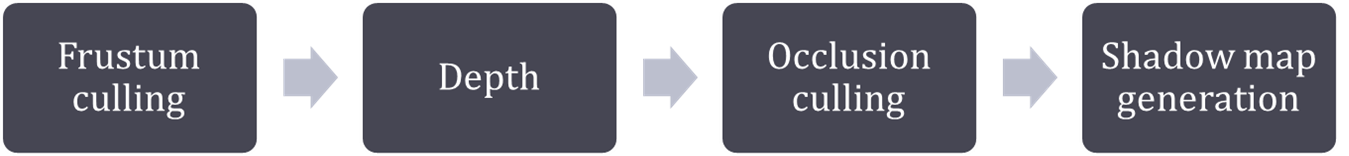
\includegraphics [scale=0.4] {my_folder/images//prepass_schema}	
		\caption{Схема этапа Pre-pass предлагаемого конвеера.} 
		\label{fig:prepass_schema}
	\end{figure}
	
	На данном этапе реализуется отбрасывание команд и наполнение буфера, требуемого для выполнения команды ExecuteIndirect. Однако, на одном и том же кадре могут требоваться команды, удовлетворяющие разным критериям, поэтому вводится несколько буферов, каждый из которых имеет разное имя:
	\begin{enumerate}[1.]
		\item All
		\item OpaqueAll
		\item TransparentsAll
		\item OpaqueFrustum
		\item OpaqueCulled
		\item TransparentCulled
	\end{enumerate}

	\subsection{Frustum culling} \label{ch3:pre_pass:frustum}
	\subsection{Depth pre-pass} \label{ch3:pre_pass:depth}
	\subsection{Occlusion culling} \label{ch3:pre_pass:occlusion}
	\subsection{Построение карт теней} \label{ch3:pre_pass:shadow_maps}